\begin{enumerate}[label=\thesection.\arabic*.,ref=\thesection.\theenumi]
\numberwithin{equation}{enumi}
\item
Sketch the Polar Plot for
\begin{align}
G(s) = \frac{1}{(1+s)(1+2s)}
\end{align}
\\
\solution  Then the given open loop Transfer Function is
\begin{align}
G(s) = \frac{1}{(1+s)(1+2s)}
\end{align}

Now we have to substitute s=j$\omega$\\
\begin{align}
G(\j\omega) = \frac{1}{(1+\j\omega)(1+2\j\omega)} 
\end{align}
\item
Then find the Magnitude of the Transfer Function
\\
\solution
\begin{multline}
      |G(\j\omega)| = \frac{1}{\sqrt{(1+(\omega^2))(1+(2\omega)^2}}
\end{multline}\\
\item
Next find the Phase of Transfer Function\\
\solution
\begin{align}
    \angle G(\j\omega) = \angle G(\j\omega)_{num} - \angle G(\j\omega)_{den}
\end{align}
\begin{multline}
    \angle G(\j\omega) = -\tan^{-1}(\omega)-\tan^{-1}(2\omega)
\end{multline}
\item
Polar plot is drawn based on this magnitude and phase of transfer function\\
\solution\\
For $\omega$=0 
\begin{align}
    |G(\j\omega)| = 1\\
    \angle G(\j\omega) = 0
\end{align}
For w= $\infty$
\begin{align}
    |G(\j\omega)| = 0\\
    \angle G(\j\omega) = -\pi
\end{align}
Next Polar Plot is drawn by varying $\omega$ from 0 to $\infty$.\\
%\usepackage{graphicx}
\begin{figure}
    \centering
    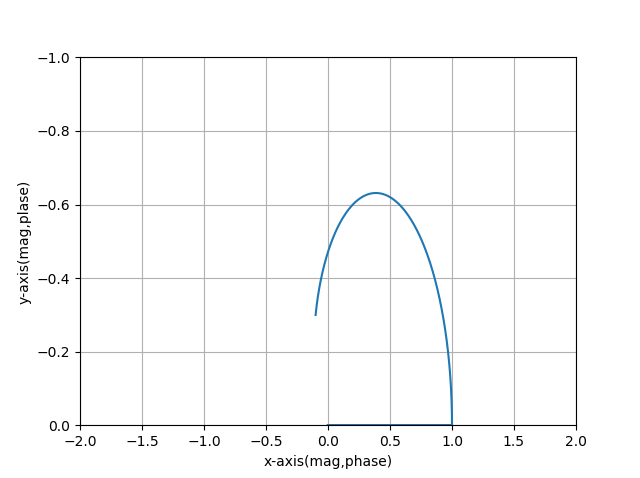
\includegraphics[width=0.7\linewidth]{ee18btech11012_1.png}
    \caption{Polar plot of given transfer function}
    \label{fig:Graph}
\end{figure}
\item
Verify the Polar Plot by running the following Code\\
\begin{lstlisting}
codes/ ee18btech11012_1.pyc
\end{lstlisting}
\item
What actually is a polar plot\\
The polar plot of the frequency response of a system is the line traced out as the frequency is changed from 0 to infinity by the tips of the phasors whose lengths represent the magnitude, i.e. amplitude gain, of the system and which are drawn at angles corresponding to their phase 
\item
Uses of Polar plots in control systems:\\
1.This is a technique which comes under frequency domain analysis.\\
2.It can capture the system behavior over the entire frequency range in a single plot.\\
3.Much easier to determine both \omega_{pc} and \omega_{gc} .\\


4.Here we will have to work with open loop transfer function G(s)H(s) (and not with closed loop transfer function and unlike Bode plot we need not required to convert G(s)H(s) to the time constant form).\\
5.polar plot tells about the magnitude and phase contribution of system at various frequency of a transfer function which is important in control systems.\\
6.Polar plot consists of concentric circles and radial lines showing the magnitude and phase of transfer function respectively.\\
7.If we know type and order of a transfer function,we can easily draw its magnitude versus phase plot using polar plot.\\
8.This is half of Nyquist plot running over positive frequencies.


\end{enumerate}
